\documentclass[11pt, a4paper]{article}
\usepackage[spanish]{babel}
\usepackage{amssymb}
\usepackage{graphicx}
\begin{document}
	\setcounter{section}{6}
	\section{Inversi\'on y polaridad}
	En esta secci\'on asumiremos conocimiento previo de inversi\'on, tambi\'en de polos y polares. Aqu\'i hay un repaso r\'apido.
	\\
	Sea $C$ un c\'irculo, con centro $O$ y radio $r$. La inversi\'on con respecto a $C$ es una transformaci\'on (De hecho, una involuci\'on) que env\'ia un punto $P$ $(\ne O)$ a un punto $P'$ en un rayo $OP$ tal que $OP \cdot OP'=r^2$.
	\linebreak
	Las inversiones ''cambian l\'ineas y c\'irculos.'' Especificamente, una l\'inea que pasa por el punto $O$ es env\'iada a s\'i misma; una l\'inea que no pasa por $O$ es env\'iada a un c\'irculo a trav\'es de $O$; un c\'irculo que pasa por O es env\'iado a una l\'inea que no pasa por $O$; Un c\'irculo que no pasa por $O$ es envi\'iado a (Posible diferente) un c\'irculo que no pasa por $O$.
	\\
	Supongamos que $P(\ne O)$ es un punto, y $\ell$ es una l\'inea pasando a trav\'es de la inversa de $P$ y tambi\'en perpendicular a $OP$, y que $P$ es el polo de $\ell$. Los mapas polares satisfacen el principio de dualidad. Por ejemplo, $P$ se encuentra en el polar de $Q$ si y solo si Q se encuentra en el polar de $P$; $\ell_1$ pasa a trav\'es del polo de $\ell_2$ si y solo si $\ell_2$ pasa a trav\'es del polo de $\ell_1$; tres polos son colineales si y solo si los tres polares correspondientes son concurrentes.
	\\\\
	Regresemos a la configuraci\'on.
	\\\\
	\textbf{Hecho 12.} Sea $ABCD$ un cuadril\'atero c\'clico con circuncentro $O$. Sea $P$ el punto de encuentro entre $AC$ y $BD$, las l\'ineas $AB$ y $CD$ se encuentran en $Q$, y las l\'ineas $DA$ y $CB$ se encuentran en $R$. Sea $M$ el punto de Miquel de $ABCD$. Entonces $P$ es el inverso de $M$ con respecto al circunc\'irculo de $ABCD$.
	\\
	$Prueba$. Dado que $P$ es la intersecci\'on de $AC$ y $BD$, bajo la inversi\'on, debe estar asignado a la intersecci\'on (Distinto a $O$) de los c\'irculos $OAC$ y $OBD$, que es $M$ (Hecho 10) $\square$
	\\
	Notemos que esto da otra prueba al Hecho 11, que dice que $O, P, M$ son colineales.
	\\
	\textbf{Hecho 13.} La l\'inea $QR$ es el polar del punto $P$.
	\\
	$Prueba$. Esto sigue del Hecho 8 y Hecho 13.
	\\
	Dado un c\'irculo $C$, decimos que un tri\'angulo es autopolar si cada lado es el polar del vertice opuesto.
	 \setcounter{footnote}{2}
	Ahora seremos capaces de probar un resultado extremadamente \'util en geometr\'ia proyectiva\footnote{Por lo que valga, aqu\'i hay un bosquejo muy r\'apido de la prueba del Hecho 14 usando geometr\'ia proyectiva: Sea un l\'inea $RP$ que interseca a $AB$ y a $BC$ en $E$ y $F$, respectivamente. Al aplicar perspectivas desde $P$ y $R$, encontramos que ($A,B;E,Q) = (C,D;F,Q) = (B,A;F,Q)$, de donde sale que $(A,B;E,Q)$ y $(C,D;F,Q)$ son ambos arm\'onicos. Luego $EF$ es es polar de $Q$, y por lo tanto $PR$ es el polar de $Q$. Paralelamente podemos mostrar que $QR$ es el polar de $P$, y $PQ$ es el polar de $Q$. Por lo tanto $PQR$ es autopolar.}.
	\newpage
	\setcounter{figure}{8}
	\textbf{Hecho 14 (Muy \'Util).} El tri\'angulo $PQR$ es autopolar con respecto al circunc\'irculo de $ABCD$
	\begin{figure}[h]
		\centering
		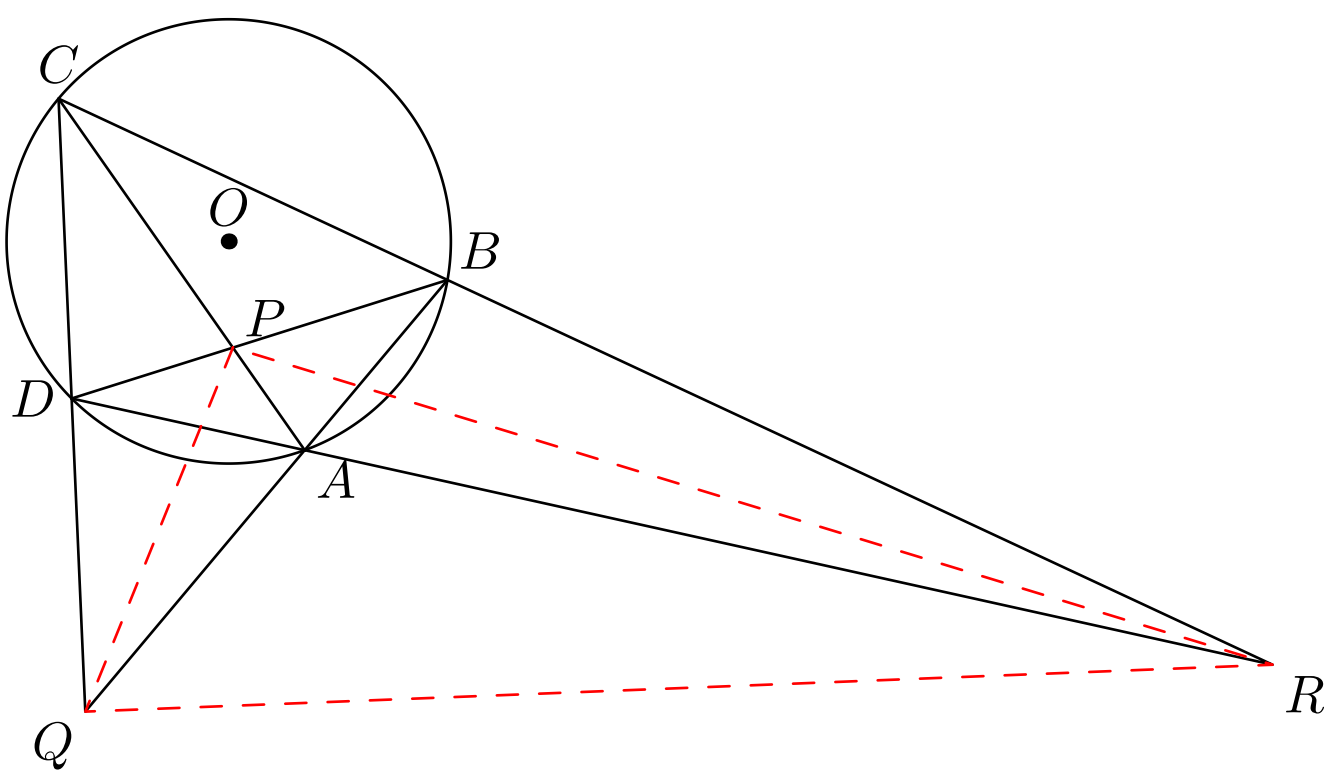
\includegraphics[scale=0.4]{p7.1 - copia}
		\caption{$PQR$ es autopolar.}
	\end{figure}
\\
	$Prueba$. No hay nada en las pruebas que requiera que tengamos $A, B, C, D$ en ese orden en el c\'irculo. Al permutar las re-etiquetas de $A, B, C, D$ podemos podemos deducir del Hecho 13 que $PR$ es el polar de $Q$, y $PQ$ es el polar de $R$. Esto nos da el resultado deseado.\\
	$\square$\\
	\textbf{Hecho 15.} $O$ es el ortocentro de $PQR$.\\
	
	$Prueba$ Esto sale inmediatamente del Hecho 14, Dado que $OX \perp \ell$ para cualquier par polo-polar $(X,\ell)$. \ $\square$
\end{document}